\documentclass[11pt]{article}
\usepackage{graphicx}
\usepackage[export]{adjustbox}
\usepackage{float}
\usepackage{amsmath}
\title{EE302 Homework 1}
\date{2018\\ March}
\author{Nail Tosun - 2094563 -Section 5\\ Electric and Electronic Engineering Departmant, METU}
\begin{document}
\maketitle
\begin{figure}[H]
  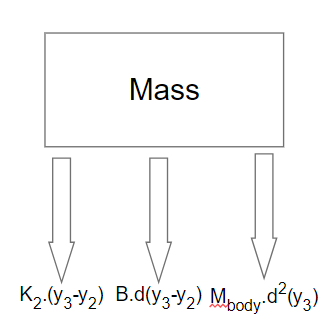
\includegraphics[scale=0.5, center]{freenody}
  \caption{ Free body diagram of body mass}
  \label{fig:zero}
\end{figure}

Assuming $y_3 > y_2 > y_1$ By Newton's second law;
\[M_{body}\ddot{y_3}=-B(\dot{y_3}-\dot{y_2})-K_2(y_3-y_2) \]
In Laplace domain with zero initial conditions;
\[(M_{body}s^2+Bs+K_2)Y_3(s)=(-Bs-K_2)Y_2(s) \]
\[Y_2(s)=\frac{M_{body}s^2+Bs+K_2}{-Bs-K_2}Y_3(s) \]

\begin{figure}[H]
  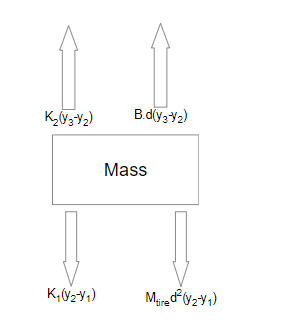
\includegraphics[scale=0.7, center]{freenody2}
  \caption{Free body diagram of tire mass}
  \label{fig:zero}
\end{figure}
 By Newton's second law;
 \[M_{tire}\ddot{y_2}=B(\dot{y_3}-\dot{y_2})+K_2(y_3-y_2)-K_1(y_2-y_1)\]
 In Laplace domain with zero initial conditions;
 \[(M_{tire}s^2+Bs+K_2+K_1)Y_2(s)=(Bs+K_2)Y_3(s)+K_1Y_1(s)\]
 Putting $Y_2(s)=\frac{M_{body}s^2+Bs+K_2}{-Bs-K_2}Y_3(s)$ into the equation;
 \[\frac{(M_{body}s^2+Bs+K_2)(M_{tire}s^2+Bs+K_2+K_1)}{-Bs-K_2}Y_3(s)=(Bs+K_2)Y_3(s)+K_1Y_1(s)\]
 $$T(s)=\frac{Y_3(s)}{Y_1(s)}$$
 \[\frac{(M_{body}s^2+Bs+K_2)(M_{tire}s^2+Bs+K_2+K_1)+(Bs+K_2)^2}{-Bs-K_2}Y_3(s)= K_1Y_1(s)\]
$$T(s)=\frac{-K_1(Bs+K_2)}{(M_{body}s^2+Bs+K_2)(M_{tire}s^2+Bs+K_2+K_1)+(Bs+K_2)^2}$$

For the state equations;
Let $z = \begin{vmatrix}
y_2 \\
\dot{y_2} \\
y_3 \\
\dot{y_3}
\end{vmatrix}$ then , $$\dot{z}=\begin{vmatrix}
\dot{y_2}\\
\ddot{y_2}\\
\dot{y_3}\\
\ddot{y_3}
\end{vmatrix}=\begin{vmatrix}
0 & 1 & 0 & 0 \\
\frac{k_2-k_1}{M_{tire}} & \frac{-b}{M_{tire}} &\frac{-k_2}{M_{tire}} & \frac{b}{M_{tire}}\\
0 & 0 & 0 & 1 \\
\frac{k_2}{M_{body}} & \frac{b}{M_{body}} & \frac{-k_2}{M_{body}} & \frac{-b}{M_{body}} \\
\end{vmatrix} \begin{vmatrix}
y_2 \\
y_3 \\
\dot{y_2} \\
\dot{y_3}
\end{vmatrix} + \begin{vmatrix}
0 \\
\frac{k_1}{M_{tire}} \\
0 \\
0
\end{vmatrix}y_1$$
$$y_3=\begin{vmatrix}
0 & 0 & 1 & 0
\end{vmatrix} \begin{vmatrix}
y_2 \\
\dot{y_2} \\
y_3 \\
\dot{y_3} \end{vmatrix}+[0]y_1$$

2)
$$\tau_0 = J\ddot{\theta_o}+B\dot{\theta_o}$$
$$\tau_0 = K_{\tau}i_m$$
$$K_{\theta}(\theta_r-\theta_o)=V_f$$
In Laplace domain;
$$V_f(s)=I_f(s)(R_f+sL_f)$$
$$V_g(s)-V_b(s)=K_gI_f(s)=(R_g+R_m)I_m(s)+(sL_g+sL_m)I_m(s) \> where \> V_b(s)=K_b\dot{\theta_o}$$
\begin{figure}[H]
  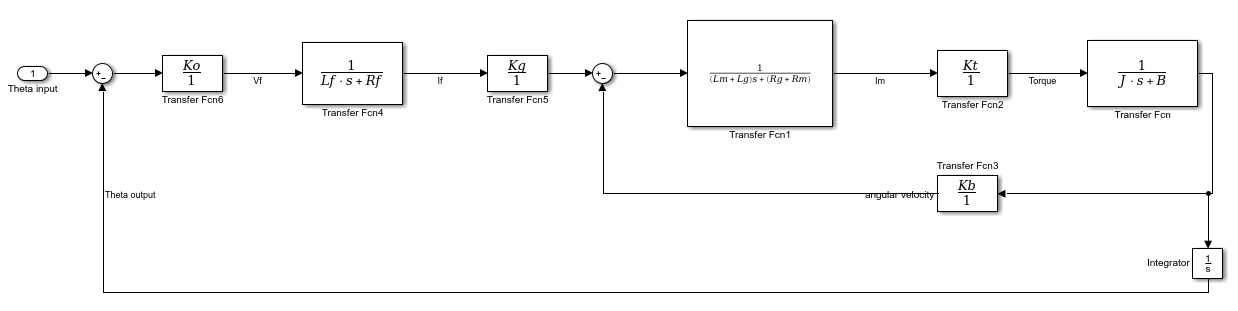
\includegraphics[scale=0.60, center]{feedback}
  \caption{Body diagram of the system}
  \label{fig:zero}
\end{figure}
$$A(s)=\frac{\frac{K_{\tau}}{(Js+B)(R_g+R_m+s(L_g+L_m)}}{1+\frac{K_b K_{\tau}}{(Js+B)(R_g+R_m+s(L_g+L_m))}}=\frac{K_{\tau}}{(Js+B)(R_g+R_m+s(L_g+L_m)+K_bK_{\tau}}$$

$$B(s)=\frac{\frac{K_{\tau}K_g K_{\theta}}{(Js+B)(R_g+R_m+s(L_g+L_m)s}}{1+\frac{K_b K_{\tau}}{(Js+B)(R_g+R_m+s(L_g+L_m)s)}}$$

B(s) is the transfer function of the system. Needed state variables number is 4 since transfer function has maximum $s^4$. 
Only second one is suitable for state variable. Because first one has input element in the vector. State variable must be linearly independent since $\tau_o=K_{tau}I_m$ fourth one is also not possible. Derivative of state variable should be linear combination of that state variable. $\dddot{\theta_o}$ is not in any equation so this is also not possible. Then state equation is following;

$$\dot{x}= \begin{vmatrix}
\dot{I_m}\\
\dot{I_f}\\
\dot{\theta_o}\\
\ddot{\theta_0}
\end{vmatrix} =\begin{vmatrix}
\frac{R_f}{L_f} & 0 & \frac{K_{\theta}}{L_f}& 0 \\
\frac{K_g}{L_g+L_m} & -\frac{R_g+R_m}{L_g+L_m} & 0 & \frac{-K_b}{L_g+L_m} \\
0 & 0 & 0 & 1\\
0 & \frac{K_{\tau}}{J} & 0 & \frac{B}{J}
\end{vmatrix} \begin{vmatrix}
I_m\\
I_f\\
\theta_o\\
\dot{\theta_0}
\end{vmatrix} + \begin{vmatrix}
\frac{K_{\theta}}{L_f}\\
0\\
0\\
0
\end{vmatrix}\theta_r$$
3)

For mechanical system; 
$$F=M\ddot{x}+B\dot{x}$$
in Laplace domain;
$$F(s)=(Ms^2+Bs)X(s)$$
In cylinder this F creates torque. Actually F is result of $\tau_2$;
$$Fr=\tau_2-K\theta_2 \> where \> \theta_2=\frac{x}{r}$$
$$T_2(s)=(Ms^2r+Bsr+\frac{K}{r})X(s)$$

For electrical system; 
\[V(s)-E_a(s)=(sL+R_a)I(s)\]
\[I(s)=\frac{V(s)-E_a(s)}{sL+R_a}\]
\[T_m(s)=K_aI(s)\]
\[T_m(s)=\frac{K_a(V(s)-E_a(s))}{sL+R_a}\]

When we do block diagram simplification for obtaining transfer function; 
\begin{figure}[H]
  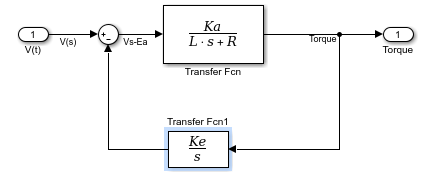
\includegraphics[width=\linewidth]{elec2}
  \caption{Electrical system block diagram}
  \label{fig:zero}
\end{figure}
\[T_m(s)=\frac{G(s)}{1+G(s)H(s)}\]
Where $G(s)=\frac{K_a}{sL+R}$ and $H(s)=\frac{K_e}{s}$
\[T_m(s)=\frac{K_a s}{s^2L+sR+K_e K_a}\]
I refer to $J_m$ to the other case (like impedance referring in transformer case) $J_m n^2$
\[T_2(s)=\frac{N_2 T_m(s)}{N_1}\]
\[T_{net}(s)=T_2(s)-K\theta_2(s)-(J+n^2J_m)s^2\theta_2(s) \>where \> \theta_2 = \frac{x}{r}\]
\[T_{net}=Fr\]
\[F(s)=(Ms^2+Bs)X(s)\]
\[T_{net}=(Ms^2+Bs)X(s)r\]
\[(Ms^2+Bs)X(s)r=\frac{N_2}{N_1}\frac{K_as}{s^2L+sR+K_e K_a}-\frac{KX(s)}{r}-\frac{(J+n^2J_m)s^2X(s)}{r^2}\]
\[T(s)=\frac{X(s)}{V(s)}\]
\[T(s)=\frac{\frac{K_mJs^2n}{(R+sL)r(Ms^2+Bs)(Jms^2+n^2(Js^2+K))}}{1+\frac{K_bsr(Ms^2+Bs)K_mJs^2n}{Js^2n(R+sL)r(Ms^2+Bs)(Jms^2+n^2(Js^2+K))}}\]

\begin{figure}[H]
  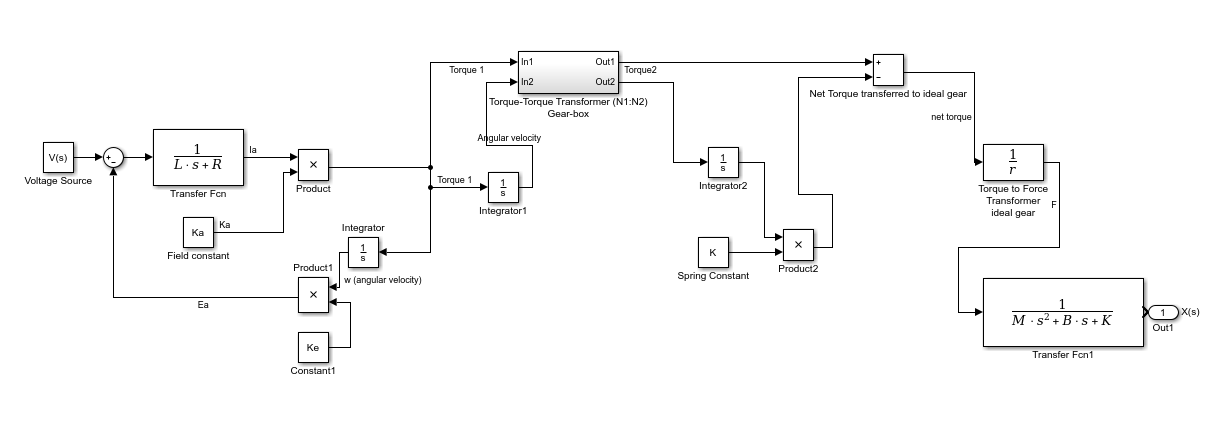
\includegraphics[width=\linewidth]{asd}
  \caption{Overall block diagram}
  \label{fig:zero}
\end{figure}

4)
\[G_5(s)\frac{G_2(s)+G_3(s)}{1+G_2(s)G_3(s)}+G_4(s)\]

\[G_6(s)=\frac{G_6(s)}{1+G_6(s)}\]
\[\frac{G_6(s)G_5(s)(G_2(s)+G_3(s))}{(1+G_6(s))(1+G_2(s)G_3(s))}+\frac{G_4(s)G_6(s)}{1+G_6(s)}\]

\[G_{overall}=\frac{\frac{G_6(s)G_5(s)(G_2(s)+G_3(s))}{(1+G_6(s))(1+G_2(s)G_3(s))}+\frac{G_4(s)G_6(s)}{1+G_6(s)}}{1+G_7(s)\frac{G_6(s)G_5(s)(G_2(s)+G_3(s))}{(1+G_6(s))(1+G_2(s)G_3(s))}+\frac{G_4(s)G_6(s)}{1+G_6(s)}}\]


\end{document}